\documentclass{beamer}
%
% Choose how your presentation looks.
%
% For more themes, color themes and font themes, see:
% http://deic.uab.es/~iblanes/beamer_gallery/index_by_theme.html
%
\mode<presentation>
{
  \usetheme{default}      % or try Darmstadt, Madrid, Warsaw, ...
  \usecolortheme{default} % or try albatross, beaver, crane, ...
  \usefonttheme{default}  % or try serif, structurebold, ...
  \setbeamertemplate{navigation symbols}{}
  \setbeamertemplate{caption}[numbered]
} 

% Packages
\usepackage[english]{babel}
\usepackage[latin1]{inputenc}
\usepackage[T1]{fontenc}
\usepackage{qrcode}

% Author
\title{Very quick introduction to Partial Differential Equations}
\author{Pablo Rodriguez-Sanchez}
\institute{Wageningen University and Research}
\date{\today}

\begin{document}

% Title
\begin{frame}
  \titlepage
  
  \begin{center}
  \qrcode{https://pabrod.github.io/intro-to-pdes-en.html}
  \end{center}
  
  \begin{center}
  pabrod.github.io/intro-to-pdes-en.html
  \end{center}
  
\end{frame}

% Disclaimer
\begin{frame}{Disclaimer}

These slides are a support for the crash course \textit{Very quick introduction to partial differential equations}, given at Wageningen University in June 2018. As a direct consequence, the slides will perform poorly if used as a self-study material.

\begin{flushright}
Pablo Rodriguez-Sanchez
\end{flushright}

\end{frame}

% Outline
\begin{frame}{Outline}
 \tableofcontents
\end{frame}

% ----------------------------------------------------------
\section{What's the difference between ODEs and PDEs?}

  \begin{frame}{What's the difference between ODEs and PDEs?}

    How are those two equations different?

    \begin{center}
    $\frac{du}{dx} = -u$
    \end{center}

    \begin{center}
    $\frac{\partial u}{\partial x} = -u$
    \end{center}

  \end{frame}

  \begin{frame}{Exercises}

    Find a function $u(x,y)$ so 

    \begin{displaymath}
    \frac{\partial u}{\partial x} =  x
    \end{displaymath}

    \pause

    and

    \begin{displaymath}
    u(0,y) = \sin y
    \end{displaymath}

    \pause

    \textbf{Solution}:

    \begin{displaymath}
    u(x,y) = \frac{x^2}{2} + \sin y
    \end{displaymath}

  \end{frame}

% ----------------------------------------------------------
\section{Introduction}

  \begin{frame}{Key ideas}

    \begin{itemize}
    \item Derivatives destroy information
        \pause
        \begin{itemize}
        \item That's why ODE problems need initial conditions to be well posed
        \end{itemize}
    \pause
    \item Partial derivatives are weapons of math destruction!
        \pause
        \begin{itemize}
        \item Problem posing with PDEs is hard
        \item PDEs are way more powerful
        \end{itemize}
    \end{itemize}

  \end{frame}

% ----------------------------------------------------------
\section{Vector calculus in a nutshell}

  \begin{frame}{Derivatives in higher dimensions}

    The \textit{nabla} operator for 2-dimensions is defined as:

    \begin{displaymath}
    \vec \nabla = \left( \frac{\partial}{\partial x}, \frac{\partial}{\partial y} \right) 
    \end{displaymath}

    \pause

    When applied to a \textit{scalar} function, it generates the gradient:

    \begin{displaymath}
    \vec {\nabla u}  = \left( \frac{\partial u}{\partial x}, \frac{\partial u}{\partial y} \right) = grad \ u
    \end{displaymath}

    \pause

    When applied to a vector function, it generates the divergence:

    \begin{displaymath}
    \vec \nabla \cdot \vec F = \frac{\partial F_x}{\partial x} + \frac{\partial F_y}{\partial y} = div \ F
    \end{displaymath}

    \pause

    When applied twice, it generates the laplacian:

    \begin{displaymath}
    \vec \nabla \cdot \vec {\nabla u}  = \nabla^2 u = \frac{\partial^2 u}{\partial x^2} + \frac{\partial^2 u}{\partial y^2}
    \end{displaymath}

  \end{frame}

% ----------------------------------------------------------
\subsection{Graphical interpretation}

  \begin{frame}{Graphical interpretation of the gradient}

    \begin{figure}
    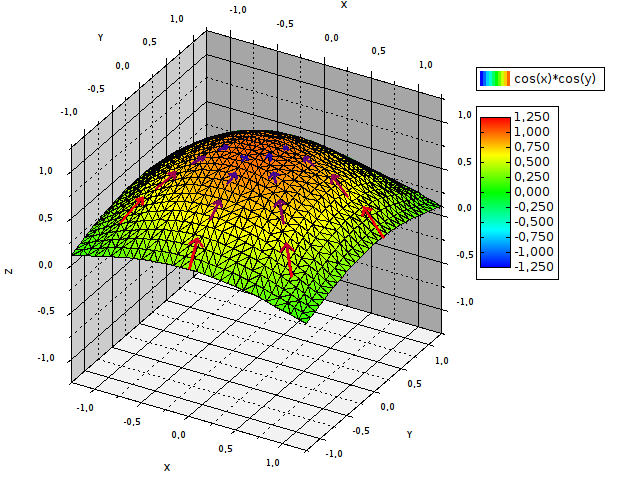
\includegraphics[scale=0.4]{img/gradient.png}
    \caption{\label{fig:gradient}Gradient points to the direction of maximum slope}
    \end{figure}

  \end{frame}

  \begin{frame}{Graphical interpretation of the divergence}

    \begin{figure}
    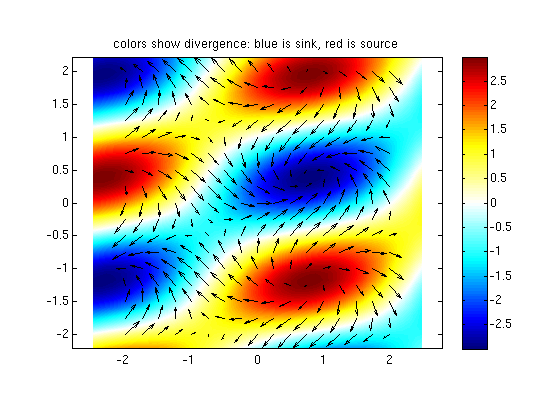
\includegraphics[scale=0.5]{img/divergence.png}
    \caption{\label{fig:divergence}Divergence is maximum in sources and minimum in sinks}
    \end{figure}

  \end{frame}

% ----------------------------------------------------------
\subsection{Summary}

  \begin{frame}{Summary of $\vec \nabla$}

    \begin{table}
    \centering
    \begin{tabular}{l|c|r}
    Operator & Shorthand & Explicit \\\hline
    Gradient & $\vec{\nabla u}$ & $\left( \frac{\partial u}{\partial x}, \frac{\partial u}{\partial y} \right) $\\
    Divergence & $\vec \nabla \cdot \vec F$ & $\frac{\partial F_x}{\partial x} + \frac{\partial F_y}{\partial y}$\\
    Laplacian & $\nabla^2 u$ & $\frac{\partial^2 u}{\partial x^2} + \frac{\partial^2 u}{\partial y^2}$
    \end{tabular}
    \caption{\label{tab:widgets}Most common generalizations of derivatives to higher dimensions.}
    \end{table}

  \end{frame}

% ----------------------------------------------------------
\section{Classical PDEs}

  \begin{frame}{Some classical PDEs}

    All classical PDEs follow the structure:

    \begin{displaymath}
    d \frac{\partial^n u}{\partial t^n} - \vec \nabla \cdot (c \vec{\nabla u}) + a u= f
    \end{displaymath}

    \pause

    \begin{table}
    \centering
    \begin{tabular}{l|c|r}
    n & Type & Some applications \\\hline
    0 & Elliptic & Electrostatics, optimization, fluid dynamics\\
    1 & Parabolic & Heat and chemical diffusion, quantum mechanics\\
    2 & Hyperbolic & Wave motion, electrodynamics
    \end{tabular}
    \caption{\label{tab:classicalPDEs}Examples of the classical PDEs.}
    \end{table}
    
  \end{frame}

  \begin{frame}{Boundary conditions}

    In 1-dimension, boundaries just need a beginning and an end

    \begin{figure}
    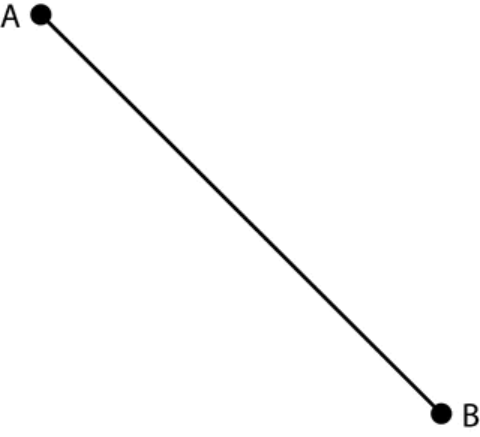
\includegraphics[scale=0.7]{img/1d-region.png}
    \caption{\label{fig:1dBoundary}Our region is delimited between A and B.}
    \end{figure}

  \end{frame}

  \begin{frame}{Boundary conditions}

    In more dimensions, boundaries have a shape

    \begin{figure}
    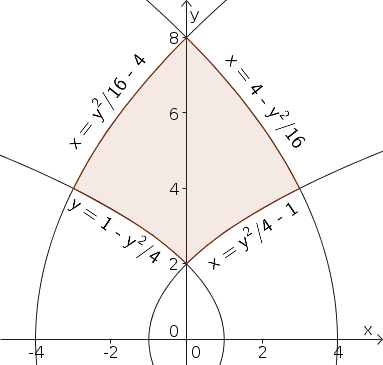
\includegraphics[scale=0.5]{img/2d-region.png}
    \caption{\label{fig:2dBoundary}Our region is... well... it's complicated.}
    \end{figure}

  \end{frame}

  \begin{frame}{Boundary conditions}

    Classical boundary conditions:

    \begin{itemize}
    \item \textbf{Dirichlet}: $u = 0$ in the border
    \pause
    \item \textbf{Von Neumann}: directional derivative in the local perpendicular of the border is zero ($\vec{\nabla u} \cdot \vec n = 0$)
    \pause
    \item \textbf{Periodic}: $u$ is equal at equivalent sides (requires defining what \textit{equivalent sides} means)
    \end{itemize}

  \end{frame}

% ----------------------------------------------------------
\section{Matlab tools}

  \begin{frame}{Matlab tools}
  
    \begin{table}
    \centering
    \begin{tabular}{l|c|r}
    Tool & Dimensions & Form \\\hline
    pdepe & u(x,t) & $c \frac{\partial u}{\partial t} = x^{-m} \frac{\partial}{\partial x}(x^m f) + s$\\
    PDE Toolbox & u(x,y,t) & $d \frac{\partial^n u}{\partial t^n} - \vec \nabla \cdot (c \vec{\nabla u}) + a u= f$
    \end{tabular}
    \caption{\label{tab:MatlabTools}PDE problems and Matlab tool.}
    \end{table}
  
  \end{frame}
  
  \begin{frame}{pdepe}
  	pdepe is used to solve equations of the following form, where $c$, $f$ and $s$ are functions of $(x,t,u, \frac{\partial u}{\partial t})$:
    
    \begin{displaymath} 
    c \frac{\partial u}{\partial t} = x^{-m} \frac{\partial}{\partial x}(x^m f) + s
    \end{displaymath}
    
    with boundary conditions:
    
    \begin{displaymath} 
    	p(x,t,u) + q(x,t) \cdot f = 0    
    \end{displaymath}
    
  	Typically, pdepe is used as:
    
    \begin{quotation}
		sol = pdepe(m, @pdefun, @icfun, @bcfun, x, t);
    \end{quotation}
    
    Where:
    
    \begin{itemize}
    
    	\item m is a real number
    	\item x and t are vectors
    	\item c, f, s = pdefun(x, t, u, DuDx)
    	\item u0 = icfun(x)
    	\item pl, ql, pr, qr = bcfun(xl, ul, xr, ur, t)
    
    \end{itemize}

    
  \end{frame}
  
  % ----------------------------------------------------------
  \subsection{Exercises}
  
  \begin{frame}{Cooling rod}
  
  In this example we will model step by step a cooling metallic rod. We know that:
  
  	\begin{itemize}
    \item The rod satisfies the heat equation
  	\item The initial temperature of the rod is zero everywhere
    \item The left border is kept at zero degrees
    \item The temperature at the right border is forced to oscillate like $u_r(t) = sin(t)$.
  	\end{itemize}
    
  \end{frame}
  
  \begin{frame}{Cooling rod}
  
  	Step 1: find c, f, s so our equation is:
    
    \begin{displaymath}
  		\frac{\partial u}{\partial t} = 0.1 \cdot \frac{\partial^2 u}{\partial x^2} 
  	\end{displaymath}
    
    \pause
    
    Step 2: find pl, ql, pr, qr so our boundary conditions are:
    
    \begin{displaymath}
    	u(0, t) =  0
  	\end{displaymath}
    
    \begin{displaymath}
    	u(1, t) =  sin(t)
  	\end{displaymath}
    
    \pause
    
    Step 3: set the initial condition $u_0(x) = 0$
  	
  \end{frame}
  
  \begin{frame}{Ripple tank}
  
  Waves in a water surface (for instance, a swimming pool) follow the wave equation:
  
    \begin{displaymath}
    	\frac{\partial^2 u}{\partial t^2} = c^2 \nabla^2 u
  	\end{displaymath}
    
  This last exercise will be entirely done with Matlab's PDE toolbox.
  
  \end{frame}

\end{document}
